% Figure 1: Phase portrait and bifurcation structure
% Created for JMLR paper (Contribution 3: Stability Landscape)
\usetikzlibrary{positioning, arrows.meta, patterns, backgrounds, fit}

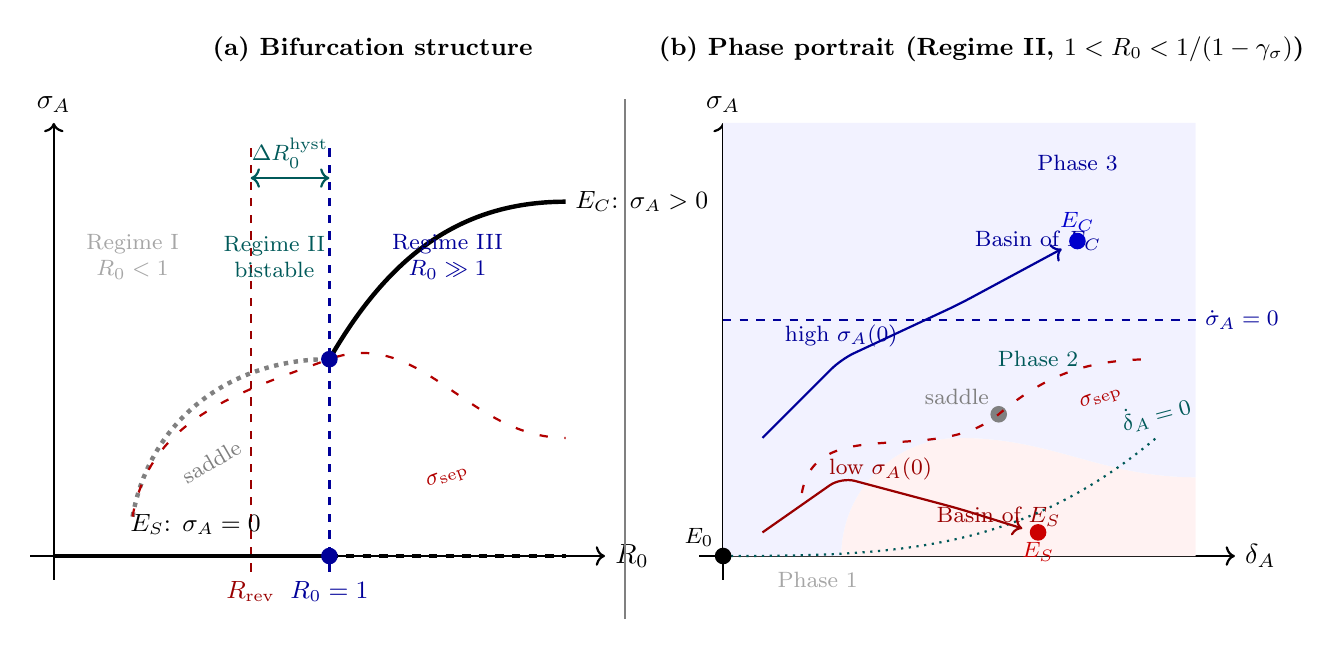
\begin{tikzpicture}[font=\sffamily]

    % ===== Panel (a): Bifurcation Diagram =====
    \begin{scope}[local bounding box=bifurcation]
        \draw[->, thick] (-0.3, 0) -- (7.0, 0) node[right] {$R_0$};
        \draw[->, thick] (0, -0.3) -- (0, 5.5) node[above] {$\sigma_A$};

        % R_0 = 1 line
        \draw[dashed, thick, blue!60!black] (3.5, -0.2) -- (3.5, 5.2);
        \node[below, font=\small, text=blue!60!black] at (3.5, -0.2) {$R_0 = 1$};

        % Reverse threshold R_rev
        \draw[dashed, thick, red!60!black] (2.5, -0.2) -- (2.5, 5.2);
        \node[below, font=\small, text=red!60!black] at (2.5, -0.2) {$R_{\mathrm{rev}}$};

        % Hysteresis band arrow
        \draw[<->, thick, teal!70!black] (2.5, 4.8) -- (3.5, 4.8);
        \node[above, font=\footnotesize, text=teal!70!black] at (3.0, 4.8) {$\Delta R_0^{\mathrm{hyst}}$};

        % Stable E_S branch (sigma=0, stable for R_0 < 1)
        \draw[ultra thick, black] (0, 0) -- (3.5, 0);
        \draw[ultra thick, black, dashed] (3.5, 0) -- (6.5, 0);
        \node[above, font=\small] at (1.8, 0.15) {$E_S$: $\sigma_A = 0$};

        % Unstable saddle branch
        \draw[ultra thick, black!50, dotted] (1.0, 0.5) to[out=80, in=180] (3.5, 2.5);
        \node[font=\footnotesize, text=black!50, rotate=30] at (2.0, 1.2) {saddle};

        % Bifurcating E_C branch (sigma > 0, stable for R_0 > 1)
        \draw[ultra thick, black] (3.5, 2.5) to[out=60, in=180] (6.5, 4.5);
        \node[right, font=\small] at (6.5, 4.5) {$E_C$: $\sigma_A > 0$};

        % Separatrix
        \draw[thick, red!70!black, loosely dashed] (1.0, 0.5) to[out=80, in=200] (3.5, 2.5)
            to[out=20, in=180] (6.5, 1.5);
        \node[font=\footnotesize, text=red!70!black, rotate=20] at (5.0, 1.0)
            {$\sigma_{\mathrm{sep}}$};

        % Label regimes
        \node[font=\footnotesize, text=gray!70, align=center] at (1.0, 3.8) {Regime I\\$R_0 < 1$};
        \node[font=\footnotesize, text=teal!70!black, align=center] at (2.8, 3.8) {Regime II\\bistable};
        \node[font=\footnotesize, text=blue!60!black, align=center] at (5.0, 3.8) {Regime III\\$R_0 \gg 1$};

        % Bifurcation point marker
        \fill[blue!60!black] (3.5, 2.5) circle (3pt);
        \fill[blue!60!black] (3.5, 0) circle (3pt);
    \end{scope}

    % ===== Panel (b): Phase Portrait (Regime II - bistable) =====
    \begin{scope}[local bounding box=portrait, shift={(8.5, 0)}]
        \draw[->, thick] (-0.3, 0) -- (6.5, 0) node[right] {$\delta_A$};
        \draw[->, thick] (0, -0.3) -- (0, 5.5) node[above] {$\sigma_A$};

        % E_S basin of attraction
        \fill[red!5] (0, 0) -- (1.5, 0) to[out=90, in=180] (3.0, 1.5)
            to[out=0, in=180] (6.0, 1.0) -- (6.0, 0) -- cycle;

        % E_C basin of attraction
        \fill[blue!5] (1.5, 0) to[out=90, in=180] (3.0, 1.5)
            to[out=0, in=180] (6.0, 1.0) -- (6.0, 5.5) -- (0, 5.5) -- (0, 0)
            -- (1.5, 0) -- cycle;

        % E_C basin label
        \node[font=\footnotesize, text=blue!60!black] at (4.0, 4.0) {Basin of $E_C$};
        \node[font=\footnotesize, text=red!60!black] at (3.5, 0.5) {Basin of $E_S$};

        % Nullclines
        % sigma nullcline
        \draw[thick, blue!60!black, dashed] (0, 3.0) -- (6.0, 3.0);
        \node[font=\footnotesize, text=blue!60!black, right] at (6.0, 3.0) {$\dot{\sigma}_A = 0$};

        % delta nullcline (approximate)
        \draw[thick, teal!70!black, dotted] (0, 0) to[out=0, in=220] (5.5, 1.5);
        \node[font=\footnotesize, text=teal!70!black, rotate=15] at (5.5, 1.8) {$\dot{\delta}_A = 0$};

        % Equilibria
        % E_0
        \fill[black] (0, 0) circle (3pt);
        \node[above left, font=\footnotesize] at (0, 0) {$E_0$};

        % E_S
        \fill[red!80!black] (4.0, 0.3) circle (3pt);
        \node[below, font=\footnotesize, text=red!80!black] at (4.0, 0.3) {$E_S$};

        % Saddle point
        \fill[black!50] (3.5, 1.8) circle (3pt);
        \node[above left, font=\footnotesize, text=black!50] at (3.5, 1.8) {saddle};

        % E_C
        \fill[blue!80!black] (4.5, 4.0) circle (3pt);
        \node[above, font=\footnotesize, text=blue!80!black] at (4.5, 4.0) {$E_C$};

        % Stable manifold (separatrix)
        \draw[thick, red!70!black, loosely dashed] (1.0, 0.8) to[out=80, in=220]
            (3.5, 1.8) to[out=40, in=180] (5.5, 2.5);
        \node[font=\footnotesize, text=red!70!black, rotate=20] at (4.8, 2.0)
            {$\sigma_{\mathrm{sep}}$};

        % Sample trajectory: falls to E_S
        \draw[->, thick, red!60!black, rounded corners=5pt]
            (0.5, 0.3) -- (1.5, 1.0) -- (3.0, 0.6) -- (3.8, 0.35);
        \node[font=\footnotesize, text=red!60!black] at (2.0, 1.1) {low $\sigma_A(0)$};

        % Sample trajectory: rises to E_C
        \draw[->, thick, blue!60!black, rounded corners=5pt]
            (0.5, 1.5) -- (1.5, 2.5) -- (3.0, 3.2) -- (4.3, 3.9);
        \node[font=\footnotesize, text=blue!60!black] at (1.5, 2.8) {high $\sigma_A(0)$};

        % Phase labels
        \node[font=\footnotesize, text=gray!70] at (1.2, -0.3) {Phase 1};
        \node[font=\footnotesize, text=teal!70!black] at (4.0, 2.5) {Phase 2};
        \node[font=\footnotesize, text=blue!60!black] at (4.5, 5.0) {Phase 3};
    \end{scope}

    % ===== Panel separator =====
    \draw[gray, thick] (7.25, -0.8) -- (7.25, 5.8);

    % ===== Panel labels =====
    \node[above, font=\small\bfseries] at ([yshift=2mm]bifurcation.north)
        {(a) Bifurcation structure};
    \node[above, font=\small\bfseries] at ([yshift=2mm]portrait.north)
        {(b) Phase portrait (Regime II, $1 < R_0 < 1/(1-\gamma_\sigma)$)};

\end{tikzpicture}
